\label{preparation_nano_ordinateur}
\par L'organigramme de la figure \ref{fig:preparation_nano_ordinateur} présente les activités qui composent la préparation du nano-ordinateur. 
\begin{figure}[H]
    \centering
    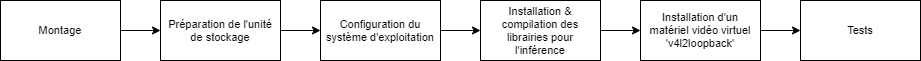
\includegraphics[width=1.0\textwidth]{preparation_nano_ordinateur}
    \caption{Préparation du nano-ordinateur}
    \label{fig:preparation_nano_ordinateur}
\end{figure}
\myparagraph{Montage}
\par Le nano ordinateur est une carte mère livrée sans aucun périphérique ni même boîtier. Vu que les performances logicielles dépendent des performances matériels, surtout pour une unité tel qu 'un nano-ordinateur où les capacités matérielles sont très limités, la première partie de l'essai a été allouée à la sélection des accessoires et périphériques qui vont permettre d'augmenter les performances, protéger et utiliser confortablement le nano-ordinateur. 
\label{montage_nano_ordinateur}
\par L'organigramme de la figure \ref{fig:montage_nano_ordinateur} présente les activités qui composent le montage du nano-ordinateur. 
\begin{figure}[H]
    \centering
    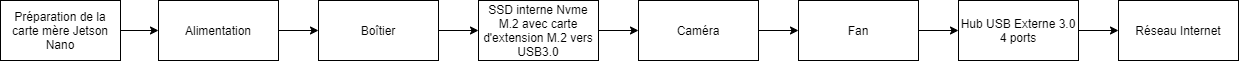
\includegraphics[width=1.0\textwidth]{montage_nano_ordinateur}
    \caption{Montage du nano-ordinateur}
    \label{fig:montage_nano_ordinateur}
\end{figure}
\mysubparagraph{Préparation de la carte mère Jetson Nano}
\begin{figure}[H]
    \centering
    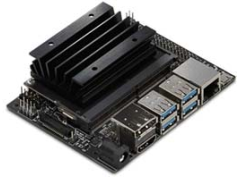
\includegraphics[width=0.5\textwidth]{jetson_nano}
    \caption{Carte mère du nano-ordinateur}
    \label{fig:jetson_nano}
\end{figure}
\par Le nano-ordinateur qui est livré dans sa boîte est uniquement une carte mère, sans unité de stockage, ni boîtier, clavier, souris, écran, capacité wifi, ou caméra. Il est uniquement livré avec un cable micro-usb qui lui permet d'être démarré avec une alimitation minimale de 5 Volt/2Amp et ne consommer que 5 Watt. Aucun système d'exploitation n'est livré non plus. Vu que de l'objectif de l'essai est de tester les capacités du nano-ordinateur et que la consommation sera de plus de 5Watt dues aux branchements de multiples périphérques, certaines "broches" sur la carte mère doivent être activées:  la broche J48 permet de brancher un adapteur d'alimentation de 5Volt 4Amp au lieu de l'alimentation micro-usb; et la broche J38 permet d'activer le PoE (Power-Over-Ethernet) afin d'hériter de l'alimentation du cable Ethernet. Aucune autre préparation sur la carte n'est nécessaire.
\mysubparagraph{Alimentation}
\begin{figure}[H]
    \centering
    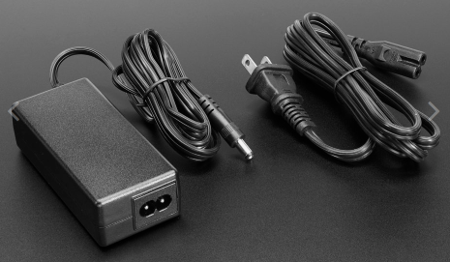
\includegraphics[width=0.5\textwidth]{alimentation}
    \caption{Adapteur 5 volt 4 amp}
    \label{fig:alimenation}
\end{figure}
\par L'alimentation du nano-ordinateur est l'élément matériel le plus important du système. De base le nano-ordinateur est livré avec un cable micro-USB, lui permettant d'être alimenté en 5Volt 2Amp. Mais le besoin en énergie augmente avec les périphériques qui s'accumulent, tel qu'une caméra. Il est prudent de choisir un adapteur 5Volt 4Amp d'un fournisseur recommandé par NVIDIA, car un changement de puissance sensible en entrée impacte le fonctionnement opérationnel du nano-ordinateur. Deux adapteurs ont été utilisés, l'un recommandé, et l'autre non, afin de tester leur performance. 
\par Dans le cadre de l'essai, l'alimentation du nano-ordinateur est utilisée pour alimenter la carte mère, qui comporte entre autre les CPUs, le GPU, le Hub USB 3.0 interne, le controleur Ethernet et le port HDMI. Mais aussi la caméra et  le ventilateur et optionellement une carte d'extension M.2 NVMe. Afin d'assister l'adapteur, un hub USB 3.0 externe a été utilisé pour brancher la souris, le clavier, et à un moment donné le dongle Wifi.
\mysubparagraph{Boîtier}
\begin{figure}[H]
    \centering
    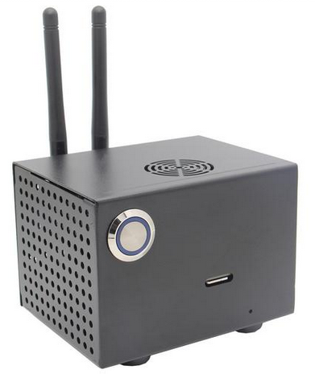
\includegraphics[width=0.45\textwidth]{boitier}
    \caption{Boitier pour le nano-ordinateur}
    \label{fig:boitier}
\end{figure}
\begin{figure}[H]
    \centering
    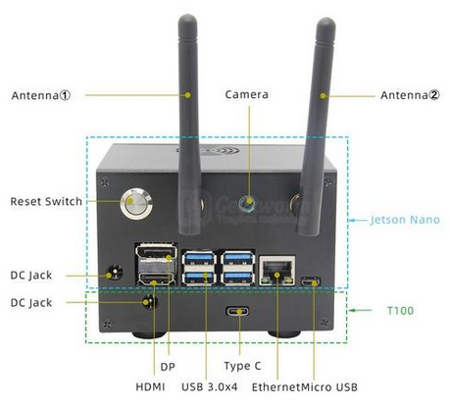
\includegraphics[width=0.5\textwidth]{boitier_back}
    \caption{Vue arrière du boitier pour le nano-ordinateur}
    \label{fig:boitier_arriere}
\end{figure}
\par Afin de protéger le nano-ordinateur durant l'essai et l'utiliser dans les conditions les plus proches de son futur mode d'opération, il a été installé dans un boîtier en métal. Le boîtier a été choisi en tenant compte qu'une carte d'extension pour un SSD interne sera installée, ainsi qu'une caméra et un ventilateur. Durant l'essai le nano-ordinateur sera manipulé très fréquemment en raison d'un manque d'espace réservé dans la maison. Le boîtier permet donc d'éviter de manipuler le matériel et les connecteurs, les protège, évitant de risquer de les briser, et donc ajouter des délais à l'essai. 
\mysubparagraph{SSD interne Nvme M.2 avec carte d'extension M.2 vers USB3.0}
\begin{figure}[H]
    \centering
    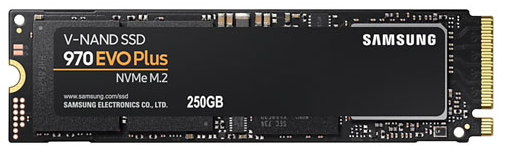
\includegraphics[width=0.5\textwidth]{Samsung 970 EVO Plus 250GB M.2 NVMe Internal Solid State Drive}
    \caption{Disque SSD NVMe M.2 interne 250GB}
    \label{fig:disquessd}
\end{figure}
\par Un disque SSD est entre 50 et 100 fois plus performant qu'une carte micro-SD. Il est aussi plus adapté pour manipuler les petits fichiers et héberger un système d'exploitation. Il est aussi plus résilient à long terme. C'est donc une option qui ne doit pas être négligée dans le contexte de tests de performance, encore plus avec un nano-ordinateur dont les capacités matériels sont limités. Néanmoins, il y a un contre-parti important dans la situation d'un nano-ordinateur: la consommation d'énergie. Un SSD interne va demander plus d'énergie qu'une carte micro-SD, et si le nano-ordinateur n'est pas capable de gérer correctement les besoins en énergie de ses extensions matériels, le SSD interne risque d'échouer en pleine opération et le nano-ordinateur devenir non fonctionnel soudainement.
\par Il y a deux choix qui ont été retenu pendant l'essai pour brancher un SSD interne au nano-ordinateur: soit via une carte d'extension M.2 MVMe, et connecté via le Hub USB, soir via une carte d'extension M.2 NVMe connecté au port PCIe interne du nano-ordinateur, normalement destinée à une carte d'extension Wifi.
\par Concernant le disque SSD M.2 NVMe connecté à la carte d'extension M.2 via le Hub USB 3.0 interne, le système L4T de NVidia (Ubuntu 18 mis à la saveur NVidia) ne supporte pas les SSD M.2 NVMe connecté au port USB. Il n'est pas reconnu / détecté, il est donc impossible de le formatter, de le partitionner, de l'utiliser. Comme il serait risqué pour l'essai de se lancer dans la recompilation du kernel du L4T, une alternative trouvée sur le développeur forum de NVidia est de passer par un adapteur M.2 MVMe connecté au port PCIe interne.
\par Malheureusement cette alternative a rapidement été abandonnée. Il a été possible de booter et installer le système d'opération sur le SSD M.2, et faire quelques tests, mais pour une raison inconnue, le système n'était pas stable et devenait non opérationnel assez rapidement, le système perdant la connexion au SSD. La durée la plus longue de stabilité observée a été de moins 30 minutes. Une hypothèse est une baisse d'énergie qui survient à un moment et qui impacte l'alimentation du SSD, chaque volt et milliampère étant important pour la stabilité du nano-ordinateur. De plus, le raccordement du cable de la carte d'extension M.2 NVMe PCIe avec le SSD M.2 NVMe est très compliquée et risqué pour le cable lui même. Une autre limitation importante est que cette solution ne permet pas d'utiliser le boîtier car le SSD M.2 ne rentre pas et ne peut même pas être fixé. 
\par Différentes options pour optimiser l'alimentation ont été explorées: utiliser un HUB USB externe et auto-alimenté; brancher un cable Ethernet au lieu d'utiliser un Dongle Wifi; allumer le ventilateur dés le démarrage du nano-ordinateur; et l'options de fournir 6Amp directement supportée par la carte mère via les pins; explorer les solutions sur les forums de discussion. 
{color{red}
Ref: https://www.kingston.com/en/community/articledetail/articleid/48543
https://geekworm.com/products/nvidia-jetson-nano-nvme-m-2-ssd-shield-t100-v1-1
\par À noter que la carte T100 est discontinuée et remplacée par T130
}
\mysubparagraph{Caméra}
\begin{figure}[H]
    \centering
    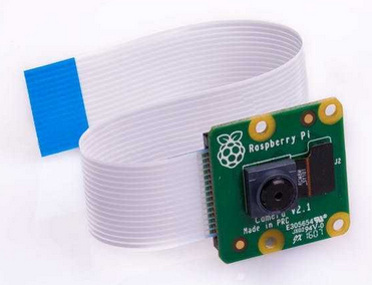
\includegraphics[width=0.40\textwidth]{camera}
    \caption{Caméra}
    \label{fig:camera}
\end{figure}
\par L'objectif du nano-ordinateur est d'être utilisé pour détecter continuellement les délimitations de la piste cyclable. Il est évident qu'une caméra doit donc faire partie du système et faire partie de l'évaluation des performances. Néanmoins, durant le déroulement de l'essai, la caméra sera très peu utilisée. En effet il n'est pas évident d'être dans un mode de développement directement sur le terrain. Un matériel vidéo virtuel sera utilisé pour simuler la caméra et alimenter l'inférence avec des vidéos pré-enregistrées, permettant ainsi d'évaluer les performances de l'inférence avec des vidéos, même si d'un point de vue performance matérielle l'utilisation ne sera pas équivalente. Les performances matérielles de l'inférence en temps réel seront évaluée avec la caméra, même si la vue de la caméra n'est pas la piste cyclable, ce qui n'est pas important pour ce test, peu importe ce qui est détecté.
\mysubparagraph{Ventilateur}
\begin{figure}[H]
    \centering
    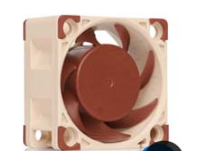
\includegraphics[width=0.35\textwidth]{fan}
    \caption{Ventilateur}
    \label{fig:fan}
\end{figure}
\par Un système informatique a besoin d'un ventilateur pour évacuer la chaleur produite par ses processeurs et les autres élément électroniques, et éviter une faute opérationnelle et des bris de matériel. L'objectif du nano-ordinateur étant d'être opérationnel continuellement, et ses éléments étant contenus dans un boîtier, il est encore plus indispensable d'installer un ventilateur. Le ventilateur choisi a pu être installé dans le boitier, même si le boîtier ne possède de support pour le fixer. Le ventilateur est capable de démarrer automatiquement au besoin, mais il est volontairement démarré manuellement dés que le nano-ordinateur est démarré. Cela évite que la chaleur ne s'accumule, qu'elle soit tout de suite ventilée à l'extérieure, évitant un risque de surchauffe, la capacité du ventilateur étant tout de même limité (petit modèle).
\mysubparagraph{Hub USB Externe 3.0 4 ports}
\begin{figure}[H]
    \centering
    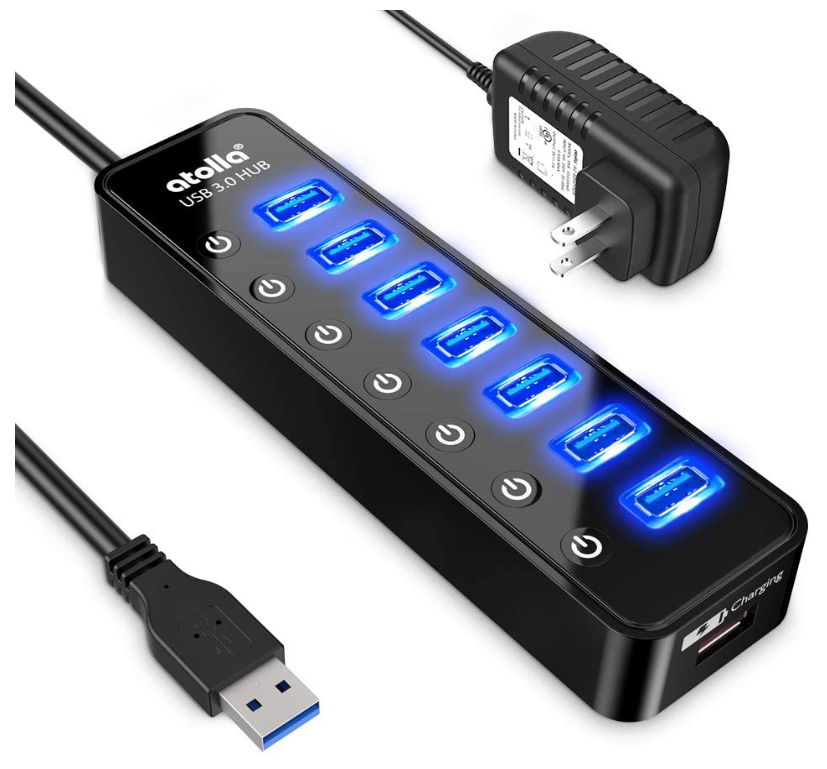
\includegraphics[width=0.4\textwidth]{Powered USB Hub 3.0, Atolla 7-Port USB Data Hub Splitter with One Smart Charging}
    \caption{Hub USB 3.0 externe autoalimenté}
    \label{fig:hubusb}
\end{figure}
\par Le nano-ordinateur comprends un hub USB 3.0 4 ports interne, les 4 ports étant connectées via le même controleur. Ce hub consomme de l'énergie pour alimenter les périphériques qui y sont connectés, comme un SSD interne ou un dongle Wifi, et gérer le échanges de données. Afin de minimiser les besoins en alimenation et optimiser le plus possible le transfer de données, la souris, le clavier et le dongle USB ont été branchées a un hub USB 3.0 externe autoalimenté. Malheureusement cette option complexifie le déploiement sur le terrain du nano ordinateur. L'alternative pour s'en passer est d'utiliser un cable Ethernet, PoE préférablement, à la place d'un dongle Wifi qui est très gourmant en terme de besoin en alimentation, et chauffe rapidement.
\mysubparagraph{Réseau Internet}
\par Le nano-ordinateur comprends un controleur Ethernet pour brancher un cable réseau et se brancher sur Internet. Selon la configuration de la carte mère, le nano-ordinateur peut hériter de l'alimentation via Ethernet (PoE), via la broche J38. Il comprends aussi aussi un port PCIe interne qui permet de brancher une carte d'extension Wifi. L'autre alternative étant de passer par un dongle USB Wifi, ou un périphérique Wifi externe connecté au port USB. 
\par Dans le cadre de cet essai, le périphérique Wifi externe USB a été utilisé en premier puisque déjà disponible. Malheureusement les performances étaient assez décevantes, le réseau Wifi à la maison n'étant pas non plus très performant dans la pièce ou le nano ordinateur était installé (table de la cuisine). Un débit d'environs 5Mbits était disponible. Par curiosité un dongle USB Wifi a été acquis, mais autant décevant. La meilleure alternative pour améliorer le déroulement de l'essai a été de tirer un cable Ethernet et d'installer un router secondaire, et de brancher le nano-ordinateur a ce nouveau router. L'accès internet a été plus stable et de bien meilleure qualité, la connexion étant d'environs 11Mbs. 
\par Le PoE n'a pas été évalué. 
\myparagraph{Préparation de l'unité de stockage}
\par Le nano-ordinateur est conçu pour fonctionner avec un système  d'exploitation hébergé sur une carte micro-SD. Il existe différentes cartes micro-SD, et certaines sont  beaucoup plus performantes que les autres. Malheureusement les cartes micro-SD ne sont pas destinées à exécuter un système d'exploitation à temps plein, et leur espérance de vie reste très limitée.  Étant donné que l'objectif du nano-ordinateur est d'être en opération continuelle à l'extérieure, l'utilisation un disque SSD interne comme alternative semble logique.
\mysubparagraph{Carte micro-sd}
\par Il existe différentes cartes micro-SD, de multiples constructeurs, et pour différents usages, mais généralement destiné pour stocker des images et vidéos directement par les appareils multimédias. Leur conception est faîte pour la manipulation de gros block de données, et non des petits fichiers. Trois cartes micro-SD 
seront évaluées: la carte micro-SD 64Gb EVO Plus (rouge; Samsung), 64Gb EVO Select (verte; Samsung), 32Gb Ultra (blanche; ScanDisk).
\mysubparagraph{Disque SSD}
\par Pour un appareil destiné a être continuellement en opération et à l'extérieure, l'unité de stockage doit être non seulement performante mais aussi endurante. Un disque SSD interne pour un nano ordinateur est soit une carte d'extension M.2 NVMe ou SATA (selon la carte d'extension), connecté au port PCIe ou USB. Les SSD internes 
Samsung 970 EVO 250GB NVMe M.2 et Samsung 860 EVO M.2 500GB SATA seront évalués. À noter qu'une carte micro-SD est tout de même nécessaire pour "bootstrapper" le système d'exploitation. Il n'est pas nécessaire d'avoir une carte micro-SD performante puisqu'elle n'est utilisée que pour démarrer le système qui se trouve sur le SSD interne. 
\myparagraph{Configuration du système d'exploitation}
\par La première fois que le système démarre, le système Ubuntu Linux For Tegra (L4T) doit être configurée avec toutes les options personnalisées (langue, clavier, timezone, etc).
\myparagraph{Installation \& compilation des librairies pour l'inférence}
\par Les librairies pour la segmentation sémantique 
d'images et de vidéos via l'inférence de modèles déjà préparées sont mises à disposition par NVIDIA via un projet dans GitHub. La documentation pour l'installation et l'inférence est disponible directement dans la page GitHub. 
\myparagraph{Installation d'un matériel vidéo virtuel 'v4l2loopback'}
\par L'inférence fournie par NVIDIA est conçue pour utiliser la caméra du nano-ordinateur. Ce qui n'est pas forcément "pratique" pour évaluer la segmentation sémantique d'une vidéo d'une piste cyclable. Heureusement un matériel vidéo virtuel permet de simuler la caméra et d'alimenter l'inférence avec une vidéo enregistrée, au lieu de la caméra. Le contre-partie concerne l'évalutation des performances:  en effet la caméra demande plus de puissance au nano-ordinateur que le simulateur logiciel.
\myparagraph{Tests}
\par Afin de s'assurer que le nano-ordinateur est prêt pour être évalué, des tests matériels et logiciels sont  effectuées une fois le système monté et stabilisé. Les résultats des tests servent de référence pour évaluer l'état de santé du nano-ordinateur. 
